% Mo Jabeen Template for docs 

\documentclass[11pt]{scrartcl} % Font size

%%%%%%%%%%%%%%%%%%%%%%%%%%%%%%%%%%%%%%%%%
% Wenneker Assignment
% Structure Specification File
% Version 2.0 (12/1/2019)
%
% This template originates from:
% http://www.LaTeXTemplates.com
%
% Authors:
% Vel (vel@LaTeXTemplates.com)
% Frits Wenneker
%
% License:
% CC BY-NC-SA 3.0 (http://creativecommons.org/licenses/by-nc-sa/3.0/)
% 
%%%%%%%%%%%%%%%%%%%%%%%%%%%%%%%%%%%%%%%%%

%----------------------------------------------------------------------------------------
%	PACKAGES AND OTHER DOCUMENT CONFIGURATIONS
%----------------------------------------------------------------------------------------

\usepackage{amsmath, amsfonts, amsthm} % Math packages

\usepackage{listings} % Code listings, with syntax highlighting

\usepackage[english]{babel} % English language hyphenation

\usepackage{graphicx} % Required for inserting images
\graphicspath{{Figures/}{./}} % Specifies where to look for included images (trailing slash required)

\usepackage{booktabs} % Required for better horizontal rules in tables

\numberwithin{equation}{section} % Number equations within sections (i.e. 1.1, 1.2, 2.1, 2.2 instead of 1, 2, 3, 4)
\numberwithin{figure}{section} % Number figures within sections (i.e. 1.1, 1.2, 2.1, 2.2 instead of 1, 2, 3, 4)
\numberwithin{table}{section} % Number tables within sections (i.e. 1.1, 1.2, 2.1, 2.2 instead of 1, 2, 3, 4)

\setlength\parindent{0pt} % Removes all indentation from paragraphs

\usepackage{enumitem} % Required for list customisation
\setlist{noitemsep} % No spacing between list items

%----------------------------------------------------------------------------------------
%	DOCUMENT MARGINS
%----------------------------------------------------------------------------------------

\usepackage{geometry} % Required for adjusting page dimensions and margins

\geometry{
	paper=a4paper, % Paper size, change to letterpaper for US letter size
	top=2.5cm, % Top margin
	bottom=3cm, % Bottom margin
	left=3cm, % Left margin
	right=3cm, % Right margin
	headheight=0.75cm, % Header height
	footskip=1.5cm, % Space from the bottom margin to the baseline of the footer
	headsep=0.75cm, % Space from the top margin to the baseline of the header
	%showframe, % Uncomment to show how the type block is set on the page
}

%----------------------------------------------------------------------------------------
%	FONTS
%----------------------------------------------------------------------------------------

\usepackage[utf8]{inputenc} % Required for inputting international characters
\usepackage[T1]{fontenc} % Use 8-bit encoding

\usepackage{fourier} % Use the Adobe Utopia font for the document

%----------------------------------------------------------------------------------------
%	SECTION TITLES
%----------------------------------------------------------------------------------------

\usepackage{sectsty} % Allows customising section commands

\sectionfont{\vspace{6pt}\centering\normalfont\upshape} % \section{} styling
\subsectionfont{\normalfont\bfseries} % \subsection{} styling
\subsubsectionfont{\normalfont\itshape} % \subsubsection{} styling
\paragraphfont{\normalfont\scshape} % \paragraph{} styling

%----------------------------------------------------------------------------------------
%	HEADERS AND FOOTERS
%----------------------------------------------------------------------------------------

\usepackage{scrlayer-scrpage} % Required for customising headers and footers

\ohead*{} % Right header
\ihead*{} % Left header
\chead*{} % Centre header

\ofoot*{} % Right footer
\ifoot*{} % Left footer
\cfoot*{\pagemark} % Centre footer

\usepackage{array}
\newcolumntype{P}[1]{>{\centering\arraybackslash}p{#1}}
 % Include the file specifying the document structure and custom commands

%----------------------------------------------------------------------------------------
%	TITLE SECTION
%----------------------------------------------------------------------------------------

\title{	
	\normalfont\normalsize
	\vspace{20pt} % Whitespace
	{\huge Basic Statistics}\\ % The meh
	\vspace{12pt} % Whitespace
	\rule{\linewidth}{2pt}\\ % Thick bottom horizontal rule
}

\author{\small Mo D Jabeen} % Your name

\date{\normalsize\today} % Today's date (\today) or a custom date


\begin{document}

\maketitle % Print the title

The example used will be the size of carrots in a farm, on the current batch.

\section{General}

\subsection{What is population and sample?}

\textbf{Population:} Entire data set, ie all the carrots.

\textbf{Sample:} A portion of the dataset, ie 30 carrots.

\subsection{What is a parameter or statistics?}

\textbf{Parameter:} Attribute from population ie mean of carrots based on all carrots.

\textbf{Statistic:} Attribute from sample ie mean from 30 carrots.\\

Random selection of the sample allows for much better statistical inference as it removes any
bias.

\subsection{What is a regression test?}

Determines if a prediction variables changes effect the outcome variable.

\subsection{What are degrees of freedom?}

The number of independent pieces of info used to calculate a statistic.

\subsection{What is the mean, expectation and standard
deviation?}

The mean is the frequency of each value occurring, multiplied by the
value all summed for each random variable.

\begin{equation}
	\overline{x} = 1/n(\Sigma fx)
\end{equation}

The expectation is the probability of each value multiplied by the
value, summed for all values. This is the value the mean tends to as the
sample size increases.

\begin{equation}
	E(x) = \Sigma x P(X=x)
\end{equation}

The variance is the average of the squared difference from the mean.

\begin{equation}
	\sigma^2 = E(X^2) - (E(X))^2
\end{equation}

The standard deviation is the square root of the variance, showing
essentially the average distance from the mean:\(\sigma\). \\

An overall shift to all data points will effect expectation and not
variance:

\begin{equation}
	E(X \pm a) = E(X) \pm a
\end{equation}

\begin{equation}
	Var(X \pm a) = Var(X)
\end{equation}

An overall multiplier to all data points effects both expectation and
variance:

\begin{equation}
	E(aX) = aE(X)
\end{equation}

\begin{equation}
	Var(aX) = a^2Var(X)
\end{equation}

\subsection{Geometric Mean}

Mean based on the product of all values, finding the nth root.

\begin{equation}
	\Pi{x}^{1/N}
\end{equation}

N is the number of values.

\subsubsection{What is it good for?}

\begin{itemize}
	\item For fraction based values ie percentages
	\item Dependant values
	\item Wildly varying values, less skewed by large data values
\end{itemize}

\section{Continuos variables}

\subsection{What is the difference between continuos and discrete
variables?}

Discrete variables are a known list of possible numbers

Continuos random variables are infinite.

\subsection{What is relative frequency density and how does it
translate to
probability?}

The relative frequency density; is a measurement of the relative
frequency over a class width (interval between two values). Relative frequency is how many times 
something happens between two values compared to number of measurements, 
class width the measurement period.

\begin{equation}
	\frac{Relative frequency}{class width} = Relative frequency density
\end{equation}

The probability density function f(x); is the relative frequency density
as n increases and the class width decreases.\\

Area under a plotted f(x) gives the probability for that range of
continuos variables.

\begin{equation}
	P(X<x) = \int_{-\infty}^{x} f(x)
\end{equation}

\begin{equation}
	\frac{d}{dx}P(X<x) = f(x)
\end{equation}

\subsection{How do you calculate the
Median?}

The median value (m) is when the probability for values above and below
are 0.5.

\begin{equation}
	\int_{m}^{\inf} f(x) = 0.5
\end{equation}

\subsection{How do you calculate a
Percentile?}

The Xth percentile is the value below which the probability is X/100:

90th percentile

\begin{equation}
	P(X<x_{90th}) = 0.9
\end{equation}

\subsection{How do you calculate the
Mean?}

If assume the a small width of delta x, the mean will be
\(\sum x(f(x)\delta(x))\) (the brackets give the probability and
multiplying by x gives the mean). As delta x tends to 0 this becomes:

\begin{equation}
	\bar{x} = \int xf(x)
\end{equation}

The population mean is then :

\begin{equation}
	\mu = \int_{-\infty}^{\infty} xf(x) dx
\end{equation}

The variance is:

\begin{equation}
	Var(x) = \int_{-\infty}^{\infty} (x -\mu)^2 f(x) dx
\end{equation}

\subsection{Inferential Statistics}

Draw conclusions and predictions based on the data.

\subsubsection{What is a confidence interval ?}

Taking into account sampling error give a range of values for the parameter and certainty percentage.

i.e. Carrots mean is [8 12cm] at 95\%.

\section{Data Validation}

\begin{itemize}
	\item Constraints
	\item Visual graphing
	\item Distribution measurements (check if mean, median and mode are similar)
	\item Good fit tests (Chi squared)
	\item Independence test (Chi squared)
	\item Check for missing or errored data
\end{itemize}

\subsection{Skew}

A dist can have right(positive), or left(negative) or zero skew. A quick check for skew is a frequency histogram.

Right skew, has a very long tail, on its right side (mean > median).\\

Normal dist has 0 skew, all symmetry dists have 0 skew.

\begin{equation}
	Pearsons\; Skew = 3*\frac{Mean-Median}{std}
\end{equation}

If skewed you can transform using square rooting, ln, log10 respectively as the skew is progressively worse.

\subsection{Kurtosis}

Measure of taildness of a distribution, how often outliers occur. Measured by checking the standardized 4th moment of a distribution.

\begin{equation}
	Kurtosis = \hat{\mu_4} = \frac{\mu_4}{\sigma^4}
\end{equation}

\(\mu_4\) is the unstandardized 4th moment.

\textbf{The above formula is biased, unbiased formula uses a correction of sample size (find online)}

\subsection{Effect Size}

Practical significance measure of if the found relationship has a real world impact.

Both Cohen d and pearsons R have guides on values showing levels of significance.

\subsubsection{What is Cohens d?}

Size of the difference between two groups.

\begin{equation}
	d = \frac{\bar{x_1} - \bar{x_2}}{s}
\end{equation}

s is the std from either a pooled data of the two groups or a control group.

\subsubsection{What is Pearsons r?}

Measures correlation by measuring variability, ie measure the effect size nutrients in the soil changes carrot length.

If positive the correlation is in the same direction and if negative its opposite.

\subsection{Coefficient of determination \(R^2\)}

How well a statistical model predicts an outcome. A goodness of fit, how close a models variance shows the dependant variables variance.\\

Can use the Pearsons correlation coefficent or least squares estimate.

\subsection{Alkaline Information Criteria}

How well a model fits the data it was generated from.\\

\textit{The best model explains the greatest amount of variation with the fewest independent variables.}\\

Method: Choose a number of models with different number of independent variables and determine which is the best.

\begin{equation}
	AIC = 2(K) * 2ln(L)
\end{equation}

K: Number of independent variables

L: Log likelihood estimate

\section{Distribution}

\subsection{General}

\begin{equation}
	X \sim N(\mu,\sigma^2)
\end{equation}

The random variable "X", belongs to "\(\sim\)" a normal distribution "N" with a specific mean and variance.

\subsubsection{What is a probability mass function?}

\textbf{PMF:} For discrete variables, it can give a calculation of the probability of an exact value.

\begin{figure}[h] % [h] forces the figure to be output where it is defined in the code (it suppresses floating)
	\centering
	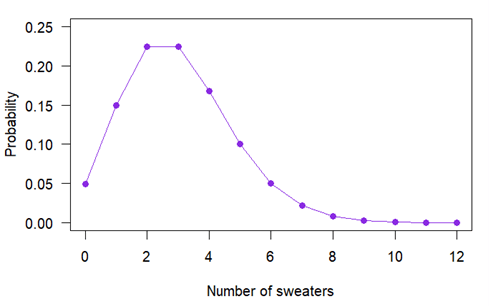
\includegraphics[width=0.5\columnwidth]{probability-example-egg-weight.png} % Example image
	\caption{PMF}
\end{figure}

\begin{table}[h] % [h] forces the table to be output where it is defined in the code (it suppresses floating)
	\centering % Centre the table
	\begin{tabular}{l l}
		\toprule
		\textit{Dist} & \textbf{Description} \\
		\midrule
		Binomial & Two states, the number of times one states shows in n trials \\
		Bernoulli & Random variable is either one of two states \\
		Discrete Uniform & probability of each state is equal \\
		Poisson & Prob an event will happen k times in a given period of time or spaces \\
		\bottomrule
	\end{tabular}
	\caption{PMF Dist}
\end{table}

\subsubsection{What is a probability density function ?}

\textbf{PDF():} For continous variables the probability of a single value is neglible and therefore
assumed at zero, instead intervals probability is calculated. Instead for a given the probability density function is used,
which measures the number of times a value is shown in a sample (its density).\\

Example: a carrot is 10cm, if the carrot shows as 10cm once in sample of 50, the PDF is 1/50.

Can determine the probability by finding multiplying a interval by its PDF.

\begin{table}[h] % [h] forces the table to be output where it is defined in the code (it suppresses floating)
	\centering % Centre the table
	\begin{tabular}{l l}
		\toprule
		\textit{Dist} & \textbf{Description} \\
		\midrule
		Normal & Centered on the mean, bell shaped\\
		Continuos Uniform & Equal intervals have equal probability \\
		Log normal & Right skewed, normal when logged \\
		Exponential & Higher prob for small values than large values.\\
		\bottomrule
	\end{tabular}
	\caption{PDF Distributions}
\end{table}

\subsection{What is the bernoulli and binomial distribution?}

Bernoulli distribution: The random variable can either be 0 or 1.\\

Binomial distribution: The random variable remains to have only two
states, this shows the probability of measuring either state x number of
times given n independent occurrences.

\subsection{Poisson Distribution}

\subsection{What is the poisson distribution
?}

\begin{itemize}
\item The random discrete variable is a count of the number of events occurring
  at random in regions of time and space. Ie radioactive particle emission or saplings in a sample of
  ground

  \begin{itemize}
  \item All events are independent
  \item No two events at the same time
  \item Over a short period of time or on a small region the probability is
    the same
  \end{itemize}
\end{itemize}

\begin{equation}
	p_x = P(X=x) = e^{-\lambda} *\lambda^{x/x!}
\end{equation}

Recurrence formula:

\begin{equation}
	P(X=x) = \lambda/x * P(X= x-1)
\end{equation}

\(\lambda\) is the mean var and \(\sqrt(\lambda)\) is the std

95\% of values are between the mean \(\pm\) 2 std

Independent Poisson random variables can be added to give another
Poisson random variable

\subsection{What is a normal distribution
?}

\textbf{Normal distribution} : Data set centered evenly about a value,
giving a bell curve.

\subsubsection{How does std related to a normal dist?}

\begin{table}[h] % [h] forces the table to be output where it is defined in the code (it suppresses floating)
	\centering % Centre the table
	\begin{tabular}{l P{2.5cm}}
		\toprule
		\textbf{STD} & \textbf{Percentage of values included (\%)}\\
		\midrule
		\(\sigma\) & 68 \\
		\(2\sigma\) & 95 \\
		\(3\sigma\) & 99.7 \\
		\bottomrule
	\end{tabular}
	\caption{std relation}
\end{table}

\subsubsection{What dist do multiple large mean samples show ?}

They will show a normal dist, even if the variable itself doesn't show a normal dist.

\subsection{Standard Normal Distribution}

Also known as z dist is a normal dist with mean = 0 and std = 1. Any normal dist can be converted
into a z dist, using the below formula to work out the z value (which calculates how many std vals
a value x from the mean is).

\begin{equation}
	z = \frac{x - \mu}{\sigma}
\end{equation}

Great reference to use as all numbers have been calculated. Can allow:

\begin{itemize}
	\item Comparisons of sample mean to population mean
	\item Compare different N dists (different mean and var)
\end{itemize}

\subsection{Chi Squared Distribution}

Not a reflection of real world distributions, but instead used for testing. Shaped by k (degrees of freedom)
, made of squared z dist with different layers of multiple of std added.

\begin{equation}
	\chi^2_{k} = (Z_1)^2 + (Z_2)^2 ... + (Z_{n\sigma})^2
\end{equation}

Hypothesis tests follow the chi squared dist under the null hypothesis. A commonly used tests is the
Pearson chi squared test. There is also a non centered chi squared dist for any skewed data.\\

Goodness of fit tests measures how well a model fits a set of observations, there is also the chi
squared Independence test.

\subsection{What is a T
Distribution?}

If the the sample size is limited and below 30, then instead of a normal
and T distribution is used.

A T dist has degrees of freedom (v) = n-1:

\begin{itemize}
\item A normal distribution has degrees of freedom v = \(\infty\)
\item n being the sample size
\end{itemize}

If the variance is unknown and n is large, Z can be adjusted to use
s\^{}2 which is an unbiased estimate of the variance. This gives two
random variables in the equation X and S:

\begin{equation}
	T = (\bar{X} - \mu)/ (S/\sqrt{n})
\end{equation}

c is the critical value depending on the distribution parameters and the
confidence interval required:

\begin{equation}
	(\bar{x} + c(s\sqrt{n}),\bar{x} - c(s\sqrt{n}))
\end{equation}

\section{Estimation}

\subsection{What is the confidence interval?}

Mean of estimate \(\pm\) variation in estimate \\

The interval is a range with a certainty value if the test was repeated in the same way the with a different sample,
the result would be the same. Essentially its a method of minimizing the sample errors effect, however does not give
a certainty on the "true value". 

\subsection{How is the confidence interval determined?}

The interval is 1-\(\alpha\), where alpha is determined arbitrarily by the field of research.

\subsection{What is the critical value?}

It is how many stds you need to go from the mean, before you reach the confidence level. To calculate the critical value
normally a transformation to a z dist is performed as the critical values are well known.

\subsection{How do you calculate the critical value?}

The critical value is the when the probability of the answer is between your interval. If converted to a z score, the
value should always be less than z value at the chosen interval.\\

\textit{Use two tailed for a 2 dimensional comparison and one tail for a 1 dimensional comparison.}\\

For a two tailed test looking for an interval of 95\% the alpha is 0.025 and the value is 1.96.

\subsection{How do you calculate the confidence interval
?}

If n observations are made from a N(\(\mu,\sigma^2)\) dist, the random variable mean from each observation will have
mean of \(\mu\) and variance of \(\frac{\sigma^2}{n}\).\\

To calculate the confidence interval of a sample mean, use the
variable Z below, where \(\bar{X}\) is random variable corresponding to the
sample mean:

\begin{equation}
	Z = (\bar{X} - \mu)/ (\sigma/ \sqrt{n})
\end{equation}

This value should then be greater or less than the critical value, giving the result.

For a normal distribution with mean 0 and std of 1 N(0,1) the confidence
interval (95\%) is:

\begin{equation}
	(\bar{x} + 1.96 (\sigma/\sqrt{n}),\bar{x} - 1.96 (\sigma/\sqrt{n}))
\end{equation}

The above interval on an average of 95\% of the time will include the
mean.

\subsection{How is s calculated ?}

s is the \textbf{sample} std, not the population which is \(\sigma\).

\begin{equation}
	s^2 = 1/(n-1) * \sum(x-\bar{x})^2
\end{equation}

\section{Statistical tests}

\subsection{What are stats tests used for?}

\begin{itemize}
	\item Determine predictor vs outcome relationship
	\item Estimate diff between two or more groups
\end{itemize}

The null hypothesis for any statistical test is that there is no relationship or difference between the two groups.\\

A number of assumptions regarding Independence, homogenity (similar variance) and normality (N()) are required to use
\textbf{parametric tests}. If they are violated non parametric tests can be used.

\subsection{How are test statistics used?}

Test statistics measure the relationship between the variables and the null hypothesis.

\subsection{What is the p value?}

P value is the probability that the observed test stat indicates the null hypothesis is true.

\subsection{What are the types of values used in stats tests?}

\begin{table}[h] % [h] forces the table to be output where it is defined in the code (it suppresses floating)
	\centering % Centre the table
	\begin{tabular}{l l}
		\toprule
		\textit{Variable} & \textbf{Description} \\
		\midrule
		Continuos & quantitative real data\\
		Discrete & quantitative integer data\\
		Ordinal & Order based data ie rankings\\
		Nominal & Names ie brand names \\
		Binary & bits \\
		\bottomrule
	\end{tabular}
	\caption{Variable types}
\end{table}

\subsection{Parametric Tests}

See table ~\ref{table:parametric} on ~\pageref{table:parametric}.

\begin{table}[h] % [h] forces the table to be output where it is defined in the code (it suppresses floating)
	\centering % Centre the table
	\begin{tabular}{P{2.5cm} P{2.5cm} P{2.5cm} P{2.5cm}}
		\toprule
		\textbf{Test} & \textbf{Predictor Var} & \textbf{Outcome Var} & \textbf{Ex} \\
		\midrule
		Simple Linear Regression & Continuos,1 predictor & Continuos, 1 outcome & How does moisture effect carrot size\\
		\midrule
		Multiple Linear Regression & Continuos, 2+ predictor & Continuos, 1 outcome & How does moisture and temp effect carrot size\\
		\midrule
		Logistic regression & Continuos, 1 predictor & Binary, 1 outcome & What is the effect of soil nutrient level on carrot death \\
		\midrule
		Paired t test & Categorical, 1 predictor & Quantitative, set of population & What is the effect of two soil types on carrot mean length from one batch\\ 
		\midrule
		Independent t test & Categorical, 1 predictor & Quantitative, sets from different population & Difference in mean carrot length from two farms\\
		\midrule
		ANOVA & Categorical, 1+ predictor & Quantitative,1 outcome & Average carrot length with three different soil types\\
		\midrule
		MANOVA & Categorical, 1+ predictor & Quantitative, 2+ outcomes & Average carrot length and width effected by soil type and seed type\\
		\midrule
		Pearsons r & Continuos, 2+ & Continuos, 1 & How are carrot length and leaf length correlated \\
		\bottomrule
	\end{tabular}
	\caption{Parametric tests}
	\label{table:parametric}
\end{table}

\subsection{Nonparametric tests}

See table ~\ref{table:nonparametric} on ~\pageref{table:nonparametric}.

\begin{table}[h] % [h] forces the table to be output where it is defined in the code (it suppresses floating)
	\centering % Centre the table
	\begin{tabular}{P{2.5cm} P{2.5cm} P{2.5cm} P{2.5cm}}		
		\toprule
		\textbf{Test} & \textbf{Predictor Var} & \textbf{Outcome Var} & \textbf{Instead of} \\
		\midrule
		Spearmens r & Quantitative & Quantitative & Pearsons r \\
		Sign test & Categorical & Quantitative & One sample t test \\
		Chi square Independence & Categorical & Categorical & Pearsons r\\
		Kruskal-Wallis H & Categorical, 3+ & Quantitative & ANOVA\\
		ANOISM & Categorical, 3+ & Quantitative 2+ & MANOVA \\
		Wilcoxon Rank Sum & Categorical, 2 & Quantitative, diff pops & Independent t test\\
		Wilcoxon Signed-rank test & Categorical 2, & Quantitative, same pop & Paired t test\\
		\bottomrule
	\end{tabular}
	\caption{Non parametric tests}
	\label{table:nonparametric}
\end{table}

\section{Hypothesis testing}

\subsection{What are the two hypothesis
statements?}

2 hypothesis are given the null (\(H_o\)) and the alternative (\(H_1\)):
- Null gives a specific parameter value - Alternative gives a range of
values

Example of a parameter used is the population mean (\(\mu\))

\subsection{How do you determine the confidence of a given null
hypothesis
?}

A normal distribution of N(\(\mu, \sigma^2\)) can be related to N(0,1)
by using \(z = (\bar{x} - \mu)/ (\sigma/\sqrt{n})\).\\

A normal distribution if the variable is adjusted to be the sample mean
\(\bar{X}\) using the mean from the null hypothesis will become
N(\(\mu_o,\sigma^2/n\)).\\

This can then be used in the form:\(P(\bar{X} > x) = P(z > (x-\mu) /\sigma)\) ; 

This is then used to calculate the confidence percentage, from the tails of the distribution
of a N(0,1).\\

\textbf{Two tailed tests gives a much more complete analysis of the data
set.}

\subsection{What are some basic terms
?}

\emph{Test statistic} : Function of data used to determine between
\(H_o\) and\(H_1\)

\emph{The critical region}: Values that lead to rejection of \(H_o\) in
favour of \(H_1\) is the critical region.

\emph{Significance level}: The probability \(H_o\) is rejected for
\(H_1\)

\subsection{What are the error types
?}

\emph{Type 1 error}: \(H_0\) is rejected for \(H_1\) however it was
correct; This is mitigated by choosing a low significance level.

\emph{Type 2 error}: \(H_o\) is accepted but incorrect.

\subsection{What is the suggested test procedure
?}

\begin{enumerate}
\item State the two hypothesis (Null and alternative)
\item Choose the appropriate test statistic and distribution
\item Choose significance level
\item Collect data
\item Analyze
\end{enumerate}

To avoid bias the sig level should be chosen before any data is
collected

If the dataset is approximately normal dist then use the standard N(0,1)

\subsection{How does confidence level relate to significance level
?}

If \(\mu_0\) is outside the range of \(\alpha\)\% confidence level, then
the significance level is (100-\(\alpha\)\%)

\subsection{Chi squared dist}

Uses the standard v degrees of freedom.

Only used for non negative random variables (generally for freq
measurements) to determine if two variables are dependant or
independent. This includes if a variable is bias by comparing it to the
expected non bias result.

\begin{figure}[h] % [h] forces the figure to be output where it is defined in the code (it suppresses floating)
	\centering
	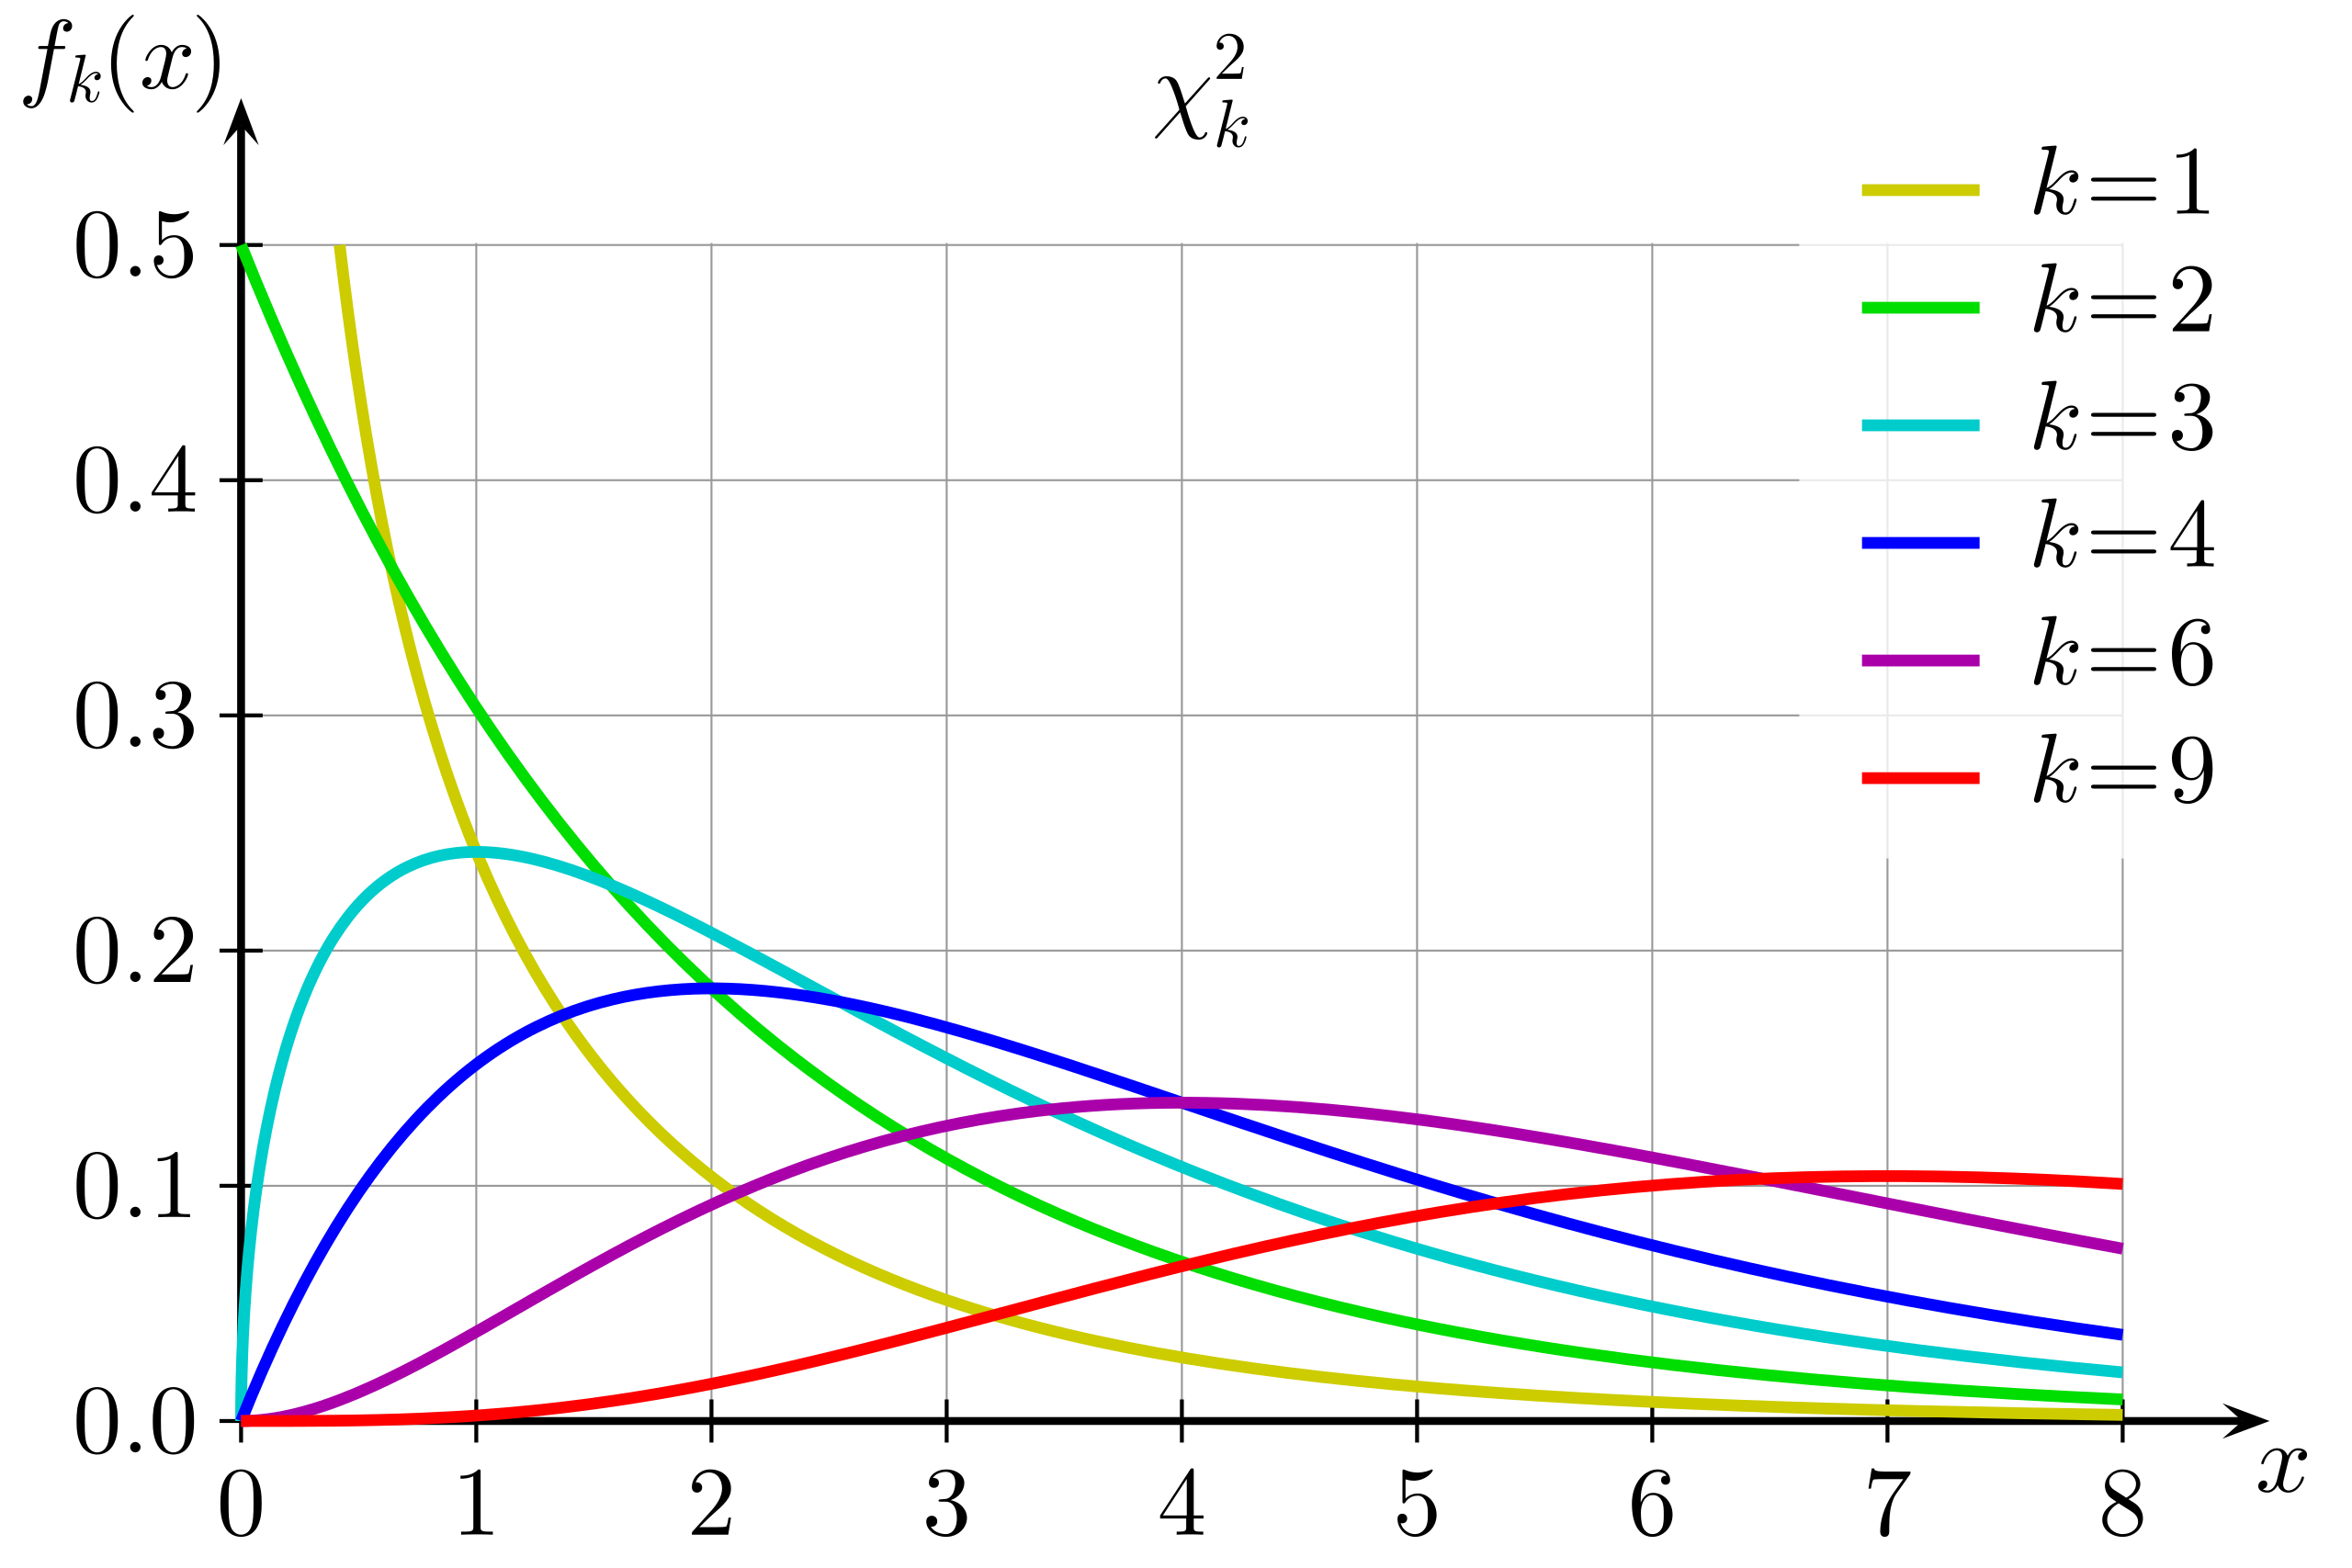
\includegraphics[width=0.5\columnwidth]{Chi-square_pdf.png} % Example image
	\caption{Chi square}
\end{figure}

As shown it is a skewed dist, as v increases the skew decreases.

\subsection{How do you test for
bias?}

The difference between the expected (non bias result) and the observed
result will indicate bias.

Both size and relative size matter:

\begin{equation}
	(O-E) * (O-E)/E = (O-E)^2/E
\end{equation}

O: Observed, E: Expected

\subsection{What value is used to determine goodness of fit between
two
models?}

\begin{equation}
	X^2 = \sum^{m}_{i=1} (O_i - E_i)^2/E_i
\end{equation}

Where m is the number of different outcomes for each model (columns).

\textbf{Large value of \(X^2\) suggest a lack of fit}

\subsection{\texorpdfstring{How does \(X^2\) relate to Chi squared
?}{How does X\^{}2 relate to Chi squared ?}}

Chi squared dist approximately shows the probability distribution of
\(X^2\), if the freq values \textgreater{} 5 :

\begin{equation}
	X^2 = \chi^2_{m-1}
\end{equation}

\subsection{What is a contingency table
?}

A table with more than two variables being measured against (two+ rows)

The degree of freedom is : \(v= (r-1)(c-1)\)

r: rows, c: columns

\textbf{If \(X^2\) is within the chi squared 95\% interval it should be
accepted as independent.}

\subsection{What should you do with a 2x2 table
?}

Can use the alternative:

\begin{equation}
	X^2 = \sum (|O-E|-0.5)^2/E
\end{equation}

\end{document}

%----------------------------------------------------------------------------------------
%	FIGURE EXAMPLE
%----------------------------------------------------------------------------------------

% \begin{figure}[h] % [h] forces the figure to be output where it is defined in the code (it suppresses floating)
% 	\centering
% 	\includegraphics[width=0.5\columnwidth]{IMAGE_NAME.jpg} % Example image
% 	\caption{European swallow.}
% \end{figure}

%----------------------------------------------------------------------------------------
% MATH EXAMPLES
%----------------------------------------------------------------------------------------

% \begin{align} 
% 	\label{eq:bayes}
% 	\begin{split}
% 		P(A|B) = \frac{P(B|A)P(A)}{P(B)}
% 	\end{split}					
% \end{align}

%----------------------------------------------------------------------------------------
%	LIST EXAMPLES
%----------------------------------------------------------------------------------------

% \begin{itemize}
% 	\item First item in a list 
% 		\begin{itemize}
% 		\item First item in a list 
% 			\begin{itemize}
% 			\item First item in a list 
% 			\item Second item in a list 
% 			\end{itemize}
% 		\item Second item in a list 
% 		\end{itemize}
% 	\item Second item in a list 
% \end{itemize}

%------------------------------------------------

% \subsection{Numbered List}

% \begin{enumerate}
% 	\item First item in a list 
% 	\item Second item in a list 
% 	\item Third item in a list
% \end{enumerate}

%----------------------------------------------------------------------------------------
%	TABLE EXAMPLE
%----------------------------------------------------------------------------------------

% \section{Interpreting a Table}

% \begin{table}[h] % [h] forces the table to be output where it is defined in the code (it suppresses floating)
% 	\centering % Centre the table
% 	\begin{tabular}{l l l}
% 		\toprule
% 		\textit{Per 50g} & \textbf{Pork} & \textbf{Soy} \\
% 		\midrule
% 		Energy & 760kJ & 538kJ\\
% 		Protein & 7.0g & 9.3g\\
% 		\bottomrule
% 	\end{tabular}
% 	\caption{Sausage nutrition.}
% \end{table}

%----------------------------------------------------------------------------------------
%	CODE LISTING EXAMPLE
%----------------------------------------------------------------------------------------

% \begin{lstlisting}[
% 	caption= Macro definition, % Caption above the listing
% 	language=python, % Use Julia functions/syntax highlighting
% 	frame=single, % Frame around the code listing
% 	showstringspaces=false, % Don't put marks in string spaces
% 	numbers=left, % Line numbers on left
% 	numberstyle=\large, % Line numbers styling
% 	]

% 	CODE

% \end{lstlisting}

%----------------------------------------------------------------------------------------
%	CODE LISTING FILE EXAMPLE
%----------------------------------------------------------------------------------------

% \lstinputlisting[
% 	caption=Luftballons Perl Script., % Caption above the listing
% 	label=lst:luftballons, % Label for referencing this listing
% 	language=Perl, % Use Perl functions/syntax highlighting
% 	frame=single, % Frame around the code listing
% 	showstringspaces=false, % Don't put marks in string spaces
% 	numbers=left, % Line numbers on left
% 	numberstyle=\tiny, % Line numbers styling
% 	]{luftballons.pl}

%------------------------------------------------

\end{document}